\chapter{Hyperdimensional computing for amino acid and sequence enconding}
\section{Encoding single amino acids into hyperdimensional vectors}
Currently, in most of the research in hyperdimensional computing, there is an emphasis on creating and assigning hyperdimensional vectors to certain concepts at random. This is useful for optimizing speed and efficiency and is not a problem for many cases such as natural language processing, where it is usually assumed that a letter does not have varying degrees of similarities to other letters in the alphabet. For protein language modeling, however, this assumption may be suboptimal since some amino acids are chemically more similar to each other than to others. We can already estimate \textit{via} many kinds of distance measures physicochemical distances between amino acids based on their physicochemical properties~\cite{physicochem} such as volume, polarity, chemical groups etc. The different similarities between amino acids are tied into the structure and thus function of amino acid sequences and shape our view of protein language. It explains why some amino acid substitutions can result in almost no phenotypical changes or on the other hand detrimental changes. Proteins have evolved to maintain their structure and function, and drastic changes in physicochemical properties can disrupt these characteristics. Therefore, amino acid substitutions that preserve the physicochemical properties of the original amino acid are more likely to be selected, resulting in a negative correlation with physicochemical distance. To account for the physicochemical information, we encoded biological information of amino acids into hyperdimensional space using amino acid embeddings from ESM-2~\cite{esm2} by simple matrix multiplications.

Instead of relying on embeddings coming from other large protein language models, we also experimented with encoding predetermined target pairwise distances onto initially random hyperdimensional vectors. First, a suitable matrix with predetermined pairwise distances has to be considered. This also implies that the matrix has to be symmetric. If we then consider the 20 essential amino acids, the problem at hand would involve a set of 20 binary vectors of length 10,000 to conform to a target distance matrix based on Hamming distance. This can be classified as a combinatorial optimization problem as it involves searching for an optimal or near-optimal configuration of binary vectors that satisfy a specific criterion. To minimize the difference between the target and actual Hamming distances for all pairs of binary vectors, we could adjust the vectors by randomly bit-flipping them until they meet the desired criteria. However, the search space in this problem is vast ($2^{10,000 x 20}$), making exhaustive search methods computationally infeasible. Thus, more efficient algorithms are needed to solve this problem such as genetic algorithms~\cite{GA}. GAs, a subfield of evolutionary algortihms, draw inspiration from the process of natural selection and emulate the evolutionary mechanisms of crossover, mutation, and selection to explore a vast search space and converge toward an optimal or near-optimal solution. The primary steps of a genetic algorithm include:
\begin{itemize}
    \item Initialization: random candidate solutions are initiated with a given population size.
    \item Crossover: combine genetic material offspring of two parents (in this case vectors). There are many recombination techniques such as single-point, multi-point and uniform crossover.
    \item Mutation: randomly alterate genes (in this case bits) to explore other possibilities of configurations and prevent premature convergence due to local optima.
    \item Evaluation: Each individual in the population (in this case a set of vectors) is assessed using a fitness function, which measures how well the solution solves the given problem.
    \item Selection: individuals from the population are selected based on their fitness to create a mating pool. Fitter individuals have a higher probability of being selected, mimicking the concept of survival of the fittest in natural evolution.
\end{itemize}
These steps are reiterated over a number of generations to obtain a set of vectors that correspond to the best fitness.

\section{Encoding proteins into hyperdimensional vectors}
State-of-the-art protein language models have the ability to gather information on long-range dependencies around a single amino acid and encode this information into neural networks and in dense numerical vectors. These models are very powerful, but as discussed earlier very resource-intensive too. To investigate the possibilities of developing embeddings on the level of amino acids, we propose a novel encoding technique within the hyperdimensional computing framework. It encodes interactions of a given amino acid in a sequence to other amino acids in its neighborhood n for a given length $n$. This method thus tries to learn and encode information about an amino acid within a sequence in an unsupervised manner.
\section{Methods}
From here on, every hyperdimensional vector is made to be 10,000-dimensional and binary unless noted otherwise. 
\subsection*{Encoding single amino acids into hyperdimensional vectors}
The last layer of the 3 billion-parameter ESM-2 model~\cite{esm2} of every amino acid was extracted, resulting in 1024-dimensional real-valued embeddings for every amino acid. To extend these into hyperdimensionality, a simple matrix multiplication has been employed: $A_{1x1024} \times B_{1024x10,000} = C_{1x10,000}$ where $A$ is a 1024-dimensional ESM-2 embedding and B a matrix of 1024 random 10,000-D vectors. The resulting vectors are then min-max scaled and rounded depending on the desired nature of the vectors. To visually assess these, the vectors for each amino acids are reduced in dimensionality \textit{via} PCA into 2 dimensions and then plotted as seen in figure~\ref{fig:AAesm}.

A \textit{BLOSUM62} substitution matrix \cite{blosum} and Grantham's distance matrix \cite{aa_evolution} were considered as pairwise similarity matrices for the GA. These were then normalized to obtain the target pairwise Hamming distances. The fitness is determined by the sum of the squared differences between the computed distance matrix of an individual and the target distance matrix. The lower the fitness value, the more optimal the individual. A genetic algorithm was implemented with the \textit{Evolutionary.jl v0.11.1}~\cite{evojl} package in \textit{Julia}. MIGHT CHANGE The population size was set to 25000 and the number of generations to 250. The mutation rate was set to 0.15 and the crossover rate to 0.2, these are respectively unusually high and low because we want to emphasize the bit-flipping and avoid recombination of vectors. HOW TO ANALYZE

To encode the neighborhood of an amino acid in a sequence, all possible pairwise interactions with the central amino acid in question in a given window are made \textit{via} binding and then all encoded into one vector \textit{via} bundling as shown figure~\ref{fig:AAtr}. Our neighborhood-encoder was tested on the human reference proteome in UniProt, entry \textit{UP000005640}, containing 20591 proteins. After all amino acids were encoded, an element-wise average was made for every amino acid. The resulting hyperdimensional vectors were kept to a real-numbered nature to not lose information for illustrative purposes.

\begin{figure}[H]
    \centering
    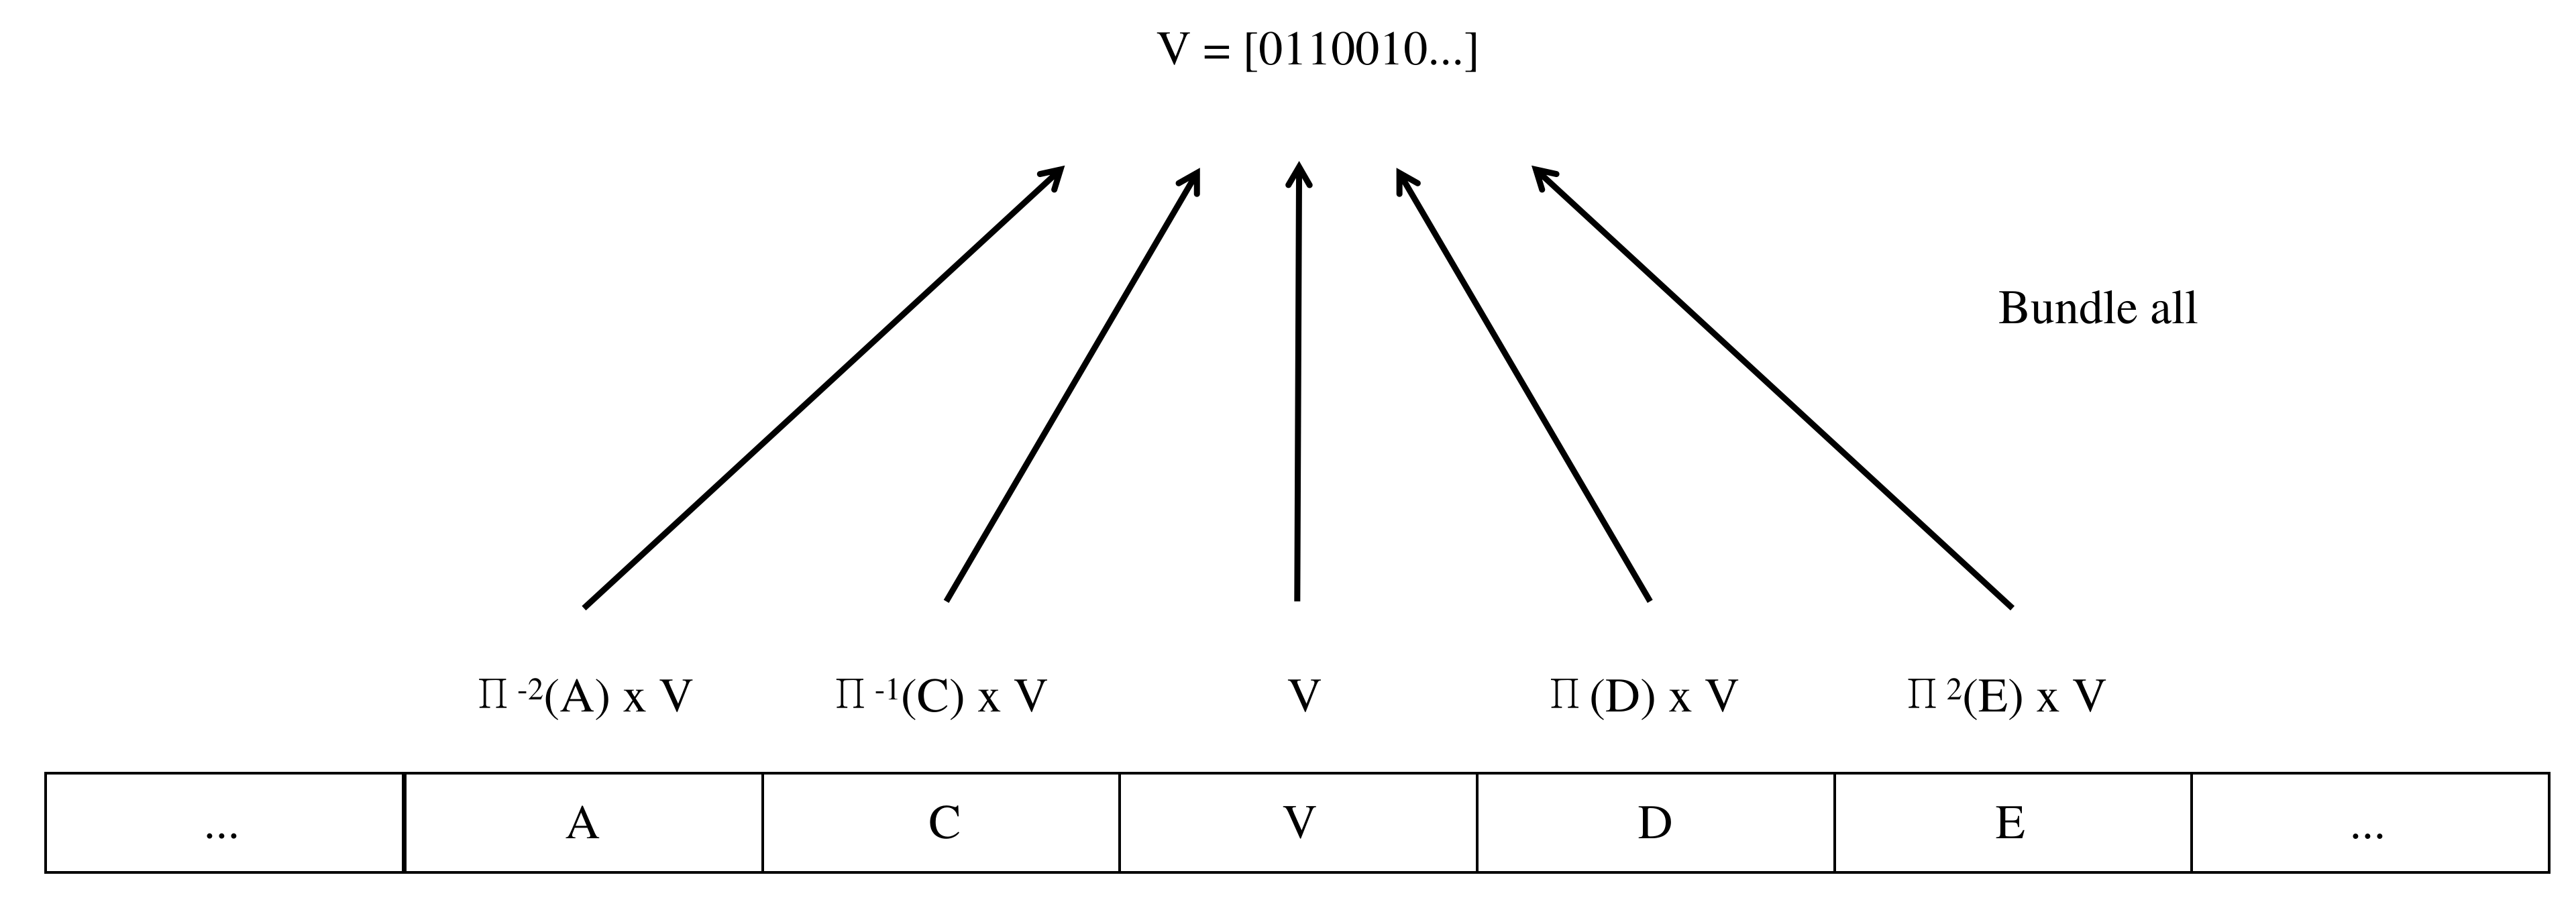
\includegraphics[scale = 0.5]{transformerlike}
    \caption{A simple demonstration of our amino acid encoder. First, HDVs are generated for every kind of amino acid, randomly or by extending ESM-2 embeddings. It considers an amino acid and all amino acids in a predetermined neigbourhood (here $n = 2$). It produces all possible interactions of the central amino acid in the window by binding and then bundles all the pairwise interactions into one hyperdimensional vector that represents the central amino acid.}
    \label{fig:AAtr}
\end{figure}


\section{Results}
At first glance, there is not much to spot in the PCA decomposition of the extended ESM-2 embeddings. Yet, if we also perform a principal component analysis on random vectors, we can see there is significantly more variance encoded into the first two principal components of the ESM embeddings (22 \%) compared to random vectors (10.5 \%, can deviate slightly depending on the run), meaning that there should be a significant amount of similarity encoded into the hyperdimensional vectors. This may be shown more clearly when used and compared in real-world problems.

\begin{figure}[H]
    \centering
    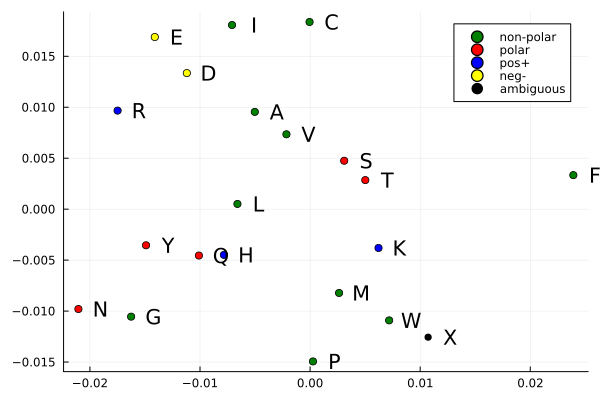
\includegraphics[scale = 0.12]{esm_emb}
    \caption{Scatter-plot of the first two principal components of ESM embeddings extended into hyperdimensionality. These PCs account for roughly 22 \% of the total variance. The amino acids are annotated and colored based on their chemical property of polarity.}\label{fig:AAesm}
\end{figure}

